\chapter{Diseño e implementación} % Main chapter title

\label{Chapter3} % Change X to a consecutive number; for referencing this chapter elsewhere, use \ref{ChapterX}


Este capítulo explica los componentes del sistema seleccionados y la descripción detallada de cada módulo de hardware y software desarrollados en el trabajo. Utilizando las definiciones y criterios descritos en capítulos anteriores, se comprende el diseño final del prototipo.

%----------------------------------------------------------------------------------------
%	SECTION 1
%----------------------------------------------------------------------------------------
\section{Diseño e implementación general del sistema}

El diseño e implementación general del sistema se subdividió en 3 partes: 

\begin{enumerate}
    \item Diseño e implementación del hardware.
    \item Diseño e implementación del firmware.
    \item Diseño e implementación de la interfaz web.
\end{enumerate}

A continuación, se describen cada una de estas partes.

%----------------------------------------------------------------------------------------
%	SECTION 2
%----------------------------------------------------------------------------------------
\section{Diseño e implementación de hardware}
\label{sec:dis_impl_hardware}

En esta sección, se describen las consideraciones de diseño del hardware del sistema. 

\subsection{Diseño del Hardware}

En la figura~\ref{fig:Arq_harware} se presenta la arquitectura del hardware desarrollado. Se incluyen todos los componentes descritos en las secciones anteriores. El sistema cuenta con 2 antenas correspondientes a la comunicación GNSS y 4G. 

Como parte de la interfaz humano-máquina, se cuenta con una pantalla LCD de 16x2, dos botones para la indicación manual de estado ocupado/desocupado y dos pilotos que permiten visualizar el estado de ocupación actual. 

En el diagrama se pueden ver los protocolos de comunicación entre módulos, entre los que se destacan:

\begin{itemize}
    \item El protocolo UART para la comunicación entre el módulo 4G SIM A7670SA por el puerto UART 0 y el módulo  GNSS Quectel L76 por el puerto UART 1. 
    \item El protocolo I2C para la comunicación con la pantalla LCD. 
\end{itemize}

Se presenta una fuente de alimentación correspondiente a una batería de 12 VDC. Debido a que los componentes del sistema operan con tensiones diferentes, se hizo necesaria la implementación de circuitos adicionales. En el diagrama, estos circuitos se denominan <<Fuente>>. Estos suplen 2 niveles de tensión distintos: 

\begin{itemize}
    \item 3,3 VDC para el Quectel L76.
    \item 5 VDC para la ESP32, el módulo SIM A7670SA y la pantalla LCD.
\end{itemize}

\begin{figure}[htbp]
	\centering
	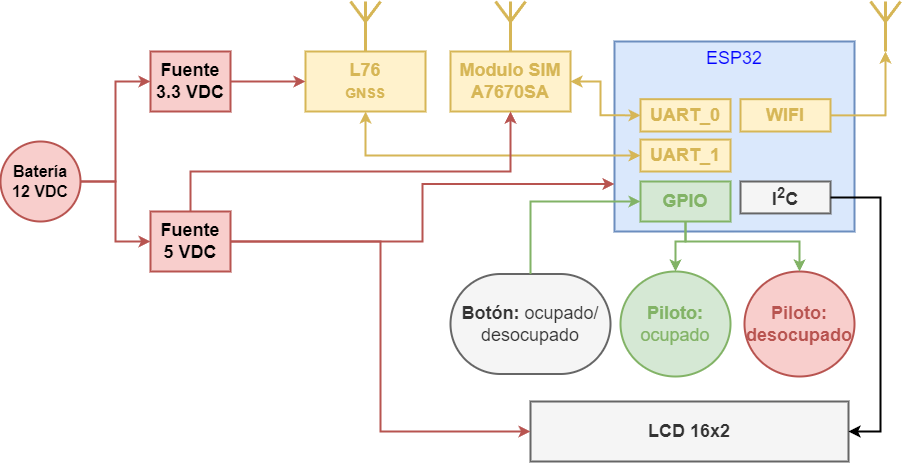
\includegraphics[width=1\textwidth]{./Figures/arquitectura_hardware_sistema.png}
	\caption{Arquitectura del hardware desarrollado.}
	\label{fig:Arq_harware}
\end{figure}



\subsection{Implementación del Hardware}

En la etapa de implementación del hardware, se trabajó en 2 placas de circuito impreso. 

\begin{enumerate}
    \item Placa base del sistema.
    \item Adaptador para el módulo Quectel L76.
\end{enumerate}



\subsubsection{Placa base del sistema}

La placa base se encarga de interconectar los módulos y periféricos principales del sistema. Por lo tanto, en el apéndice~\ref{AppendixA} se presenta el circuito esquemático correspondiente a esta implementación. En esta se empleó el regulador MIC29302WU, con una configuración de ajuste por defecto en 5 VDC, para la alimentación de la ESP32, del módulo SIM A7670SA, la placa adaptador para el módulo Quectel L76 y la pantalla LCD. En la figura~\ref{fig:placa_base_2d} se puede apreciar el diseño final del PCB en un modelo de dos dimensiones. Además, en la figura~\ref{fig:placa_base_3d} se observa el modelo en tres dimensiones. 

Los componentes U1, U2 y H3, corresponden a las ranuras donde se conectan la ESP32 DevKit V4, el adaptador para el módulo Quectel L76, y el módulo SIM A7670SA, respectivamente. Las terminales marcadas con CN6 y CN7 permiten la conexión de los pilotos que indican la ocupación de la cava. Las terminales CN4 y CN5 corresponden a las conexiones de los botones de que dispondrá el operario de la cava para la indicación de la ocupación. Por otro lado, las terminales CN2 y CN3 corresponden a la interfaz I2C y la alimentación de la pantalla LCD, respectivamente. La terminal CN1 corresponde a la entrada de alimentación del sistema. Finalmente, las terminales CN9 y CN11 externalizan los pines GPI 34 y GPI 35, y GPIO 5 y GPIO 18 de la ESP32, respectivamente; esto para facilitar, en una etapa posterior, la agregación de nuevas funcionalidades. 

\begin{figure}[htbp]
	\centering
	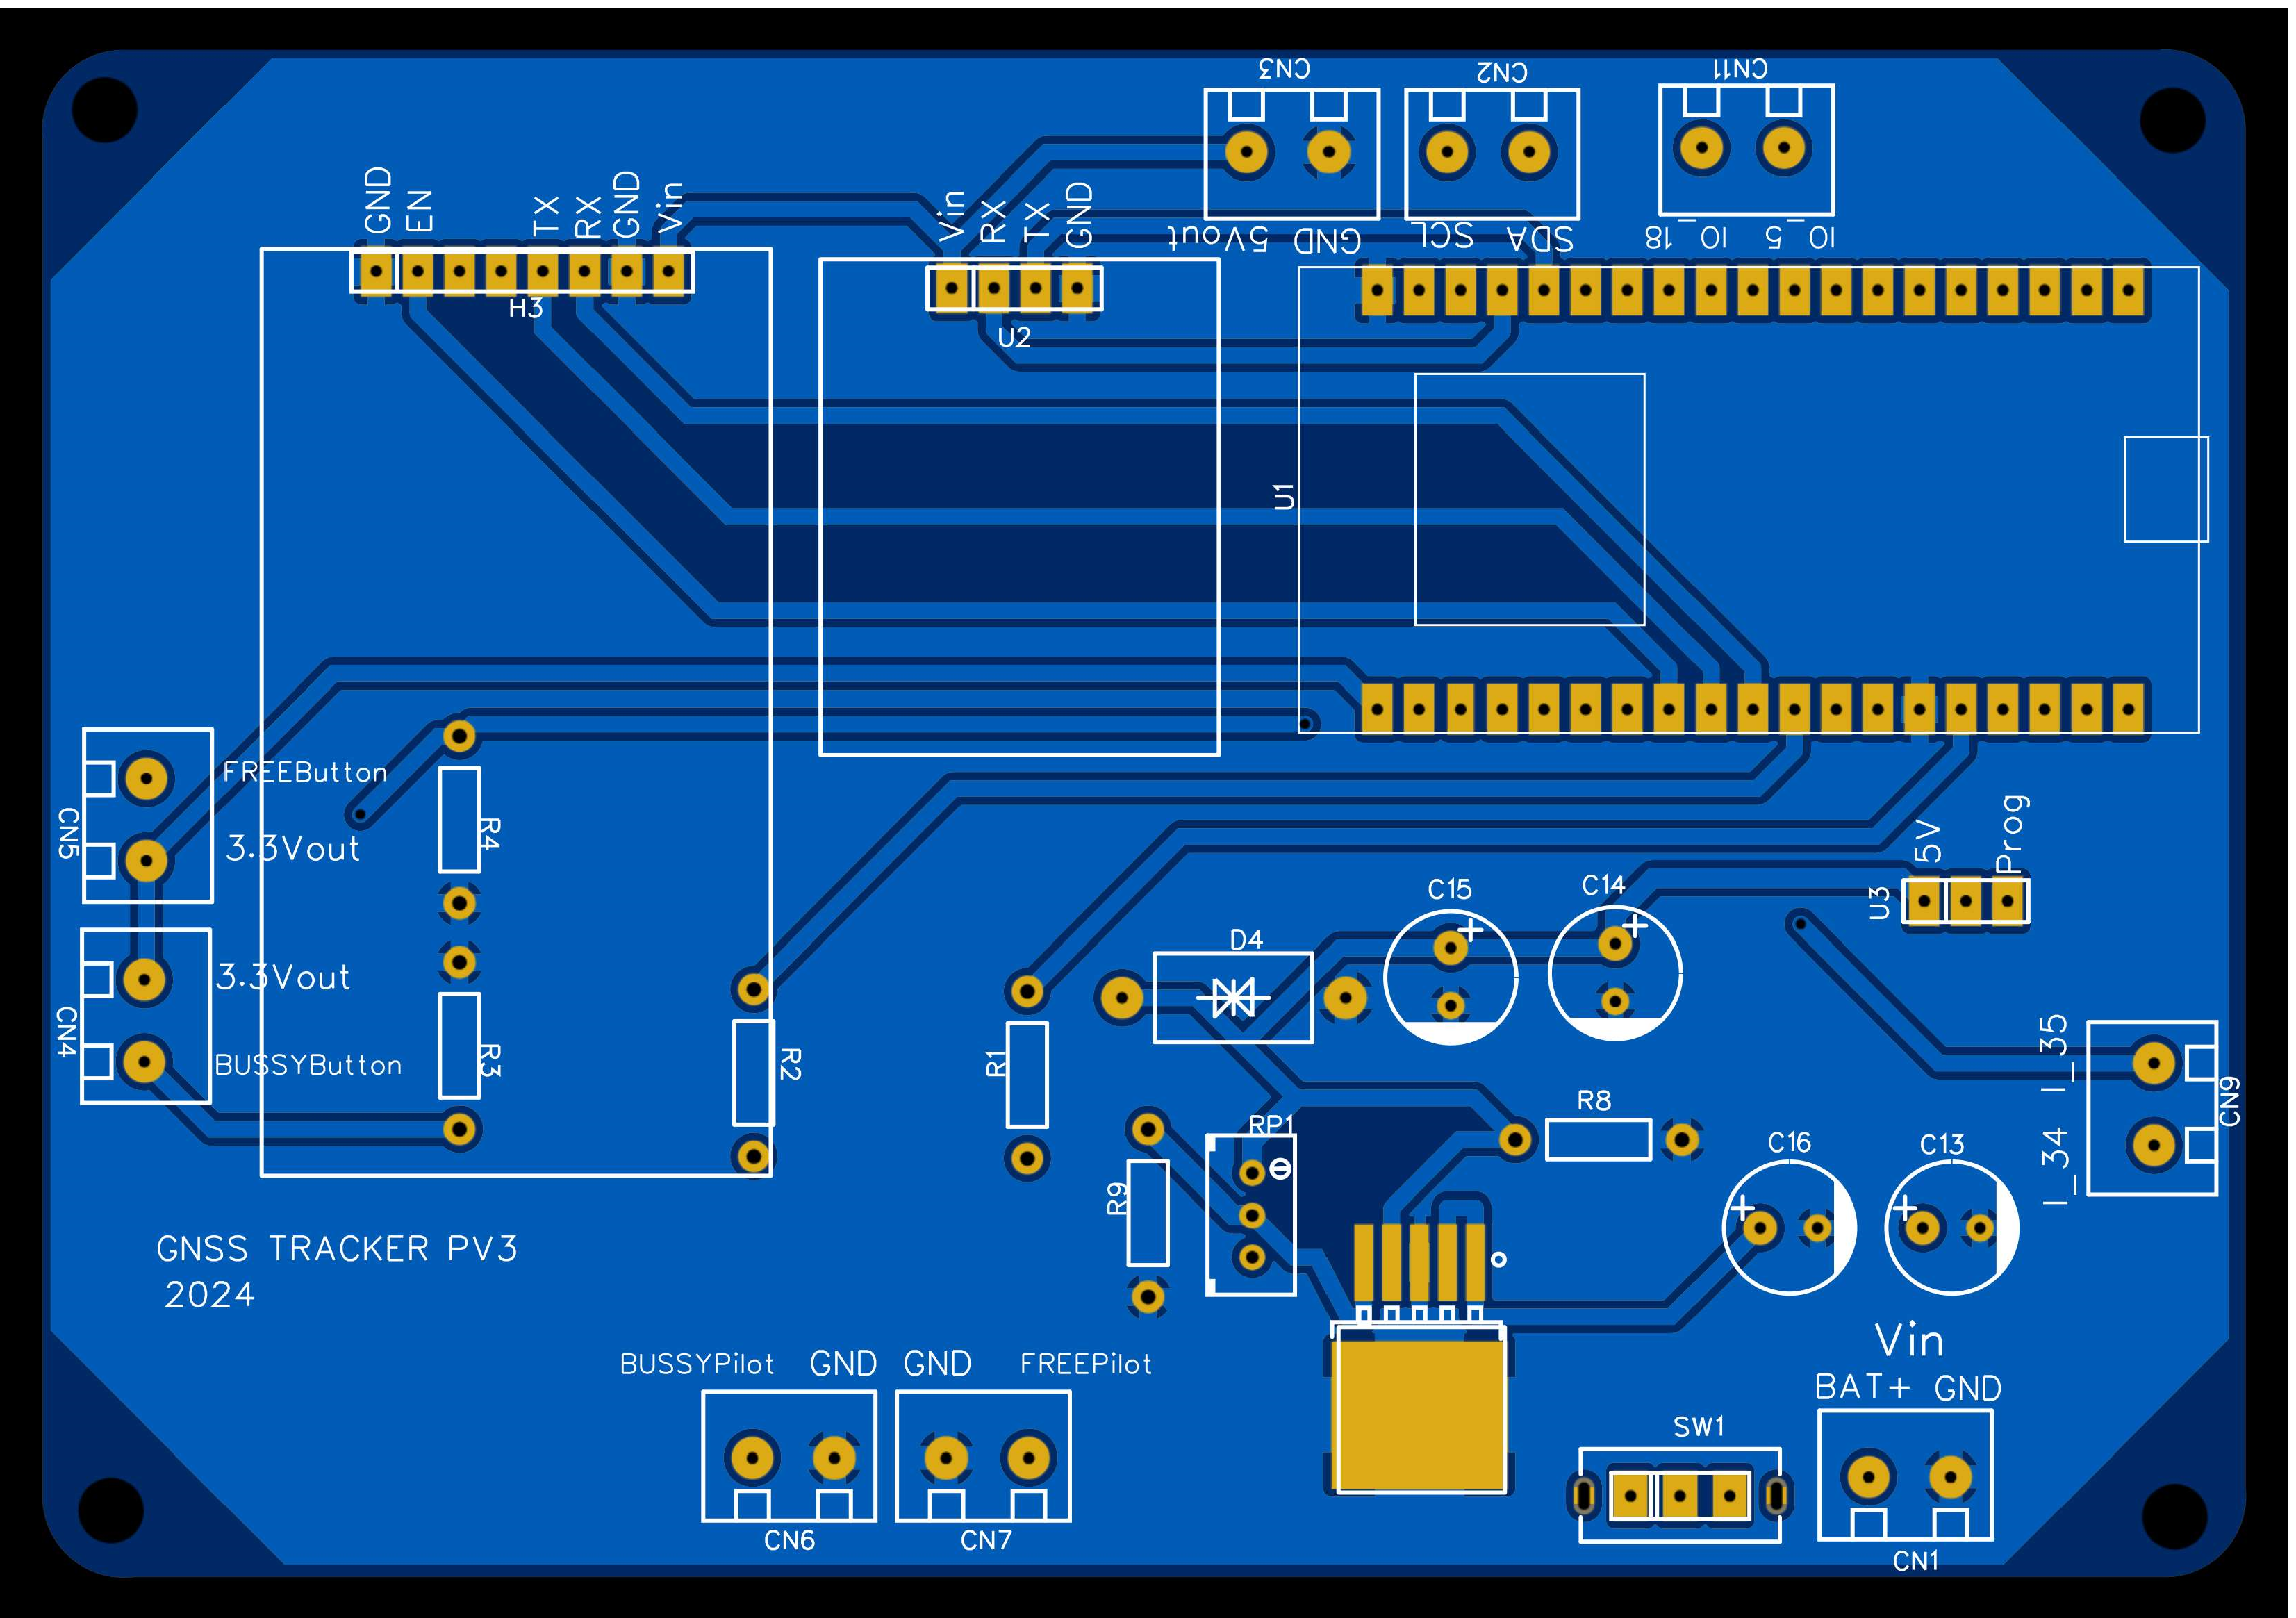
\includegraphics[width=.8\textwidth]{./Figures/PCB_TFE_Modelo_2D.png}
	\caption{Modelo 2D de la placa base del sistema.}
	\label{fig:placa_base_2d}
\end{figure}

\begin{figure}[htbp]
	\centering
	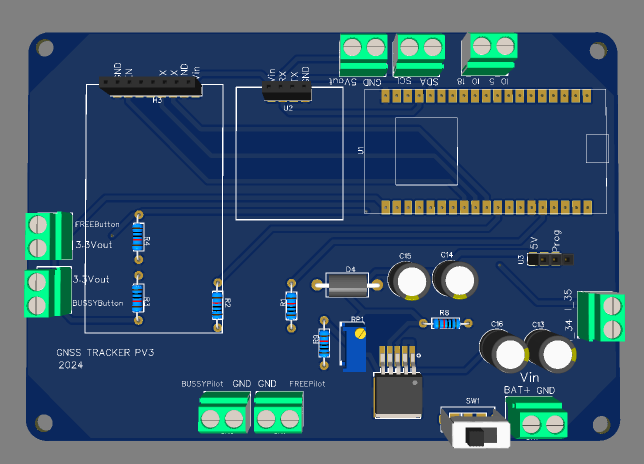
\includegraphics[width=.8\textwidth]{./Figures/PCB_TFE_Modelo_3D.png}
	\caption{Modelo 3D de la placa base del sistema.}
	\label{fig:placa_base_3d}
\end{figure}


\subsubsection{Adaptador para el módulo Quectel L76}

El circuito esquemático del adaptador L76 se encuentra en la figura~\ref{fig:adap_L76}. En este esquemático se puede observar la fuente de 3.3 VDC de entrada de alimentación, la conexión UART y la conexión entre el módulo y el microcontrolador ESP32.  

En las figuras~\ref{fig:adap_L76_2d} y~\ref{fig:adap_L76_3d}, se muestran los modelos 2D y 3D del circuito diseñado. 

\begin{figure}[htbp]
	\centering
	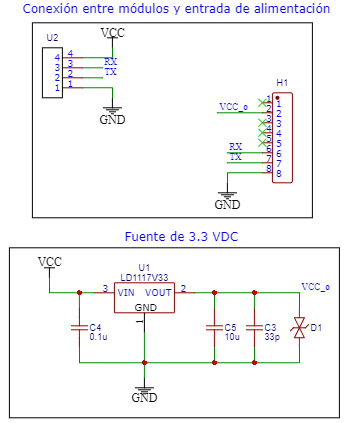
\includegraphics[width=.6\textwidth]{./Figures/QL76_Esquematico.png}
	\caption{Esquemático del adaptador L76.}
	\label{fig:adap_L76}
\end{figure}

\begin{figure}[htbp]
	\centering
	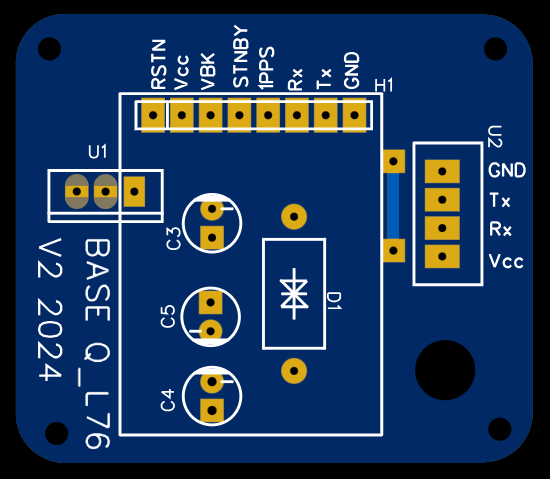
\includegraphics[width=.4\textwidth]{./Figures/QL76_modelo_2d_sup.png}
	\caption{Modelo 2D del adaptador L76.}
	\label{fig:adap_L76_2d}
\end{figure}

\begin{figure}[htbp]
	\centering
	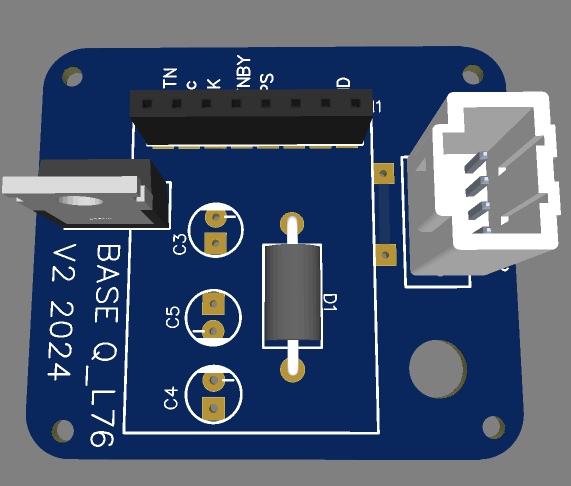
\includegraphics[width=.4\textwidth]{./Figures/QL76_modelo_3d_sup.png}
	\caption{Modelo 3D del adaptador L76.}
	\label{fig:adap_L76_3d}
\end{figure}



%----------------------------------------------------------------------------------------
%	SECTION 3
%----------------------------------------------------------------------------------------
\section{Diseño e implementación del firmware}

En esta sección se presentan las consideraciones de diseño y el proceso de implementación del firmware. 

\subsection{Diseño del firmware}

El propósito del firmware desarrollado es satisfacer los requerimientos de conectividad, administración del hardware e interfaz con el usuario. A continuación se describen las principales funcionalidades del firmware: 

\begin{enumerate}
 \item Realizar las funciones de conexión a Internet a través de la red celular, a través de la comunicación por comandos AT-UART con el módulo SIM A7670SA, para asegurar la conexión con el \textit{Broker} MQTT.
 \item Comunicación a través de tramas NMEA por el puerto UART con el módulo Quectel L76. Para la recepción e interpretación de los datos de geolocalización de las constelaciones GPS y BeiDou.  
 \item Monitoreo de los botones de ocupación a través de interrupciones y visualización de los estados de ocupación a través de los pilotos. 
 \item Generación de interfaz visual a través de la comunicación I2C con la pantalla LCD 16x2. 
 \item Administración de la energía del sistema a través de los modos de bajo consumo. 
 \item Administración de los recursos del microcontrolador a través de la implementación del sistema operativo en tiempo real FreeRTOS. 
\end{enumerate}

\subsubsection{Arquitectura del firmware}
\label{sec:arquitectura_firmware}

De acuerdo con lo planteado anteriormente, en la figura~\ref{fig:arq_firmware} se presenta un diagrama de componentes UML, que representa la arquitectura del sistema general, con énfasis en los componentes del firmware. 

En este diagrama (figura~\ref{fig:arq_firmware}) se representan como subsistemas (\textit{Subsystem}) los componentes de hardware como la ESP32, la pantalla LCD, el módulo 4G SIM A7670SA, los botones y los pilotos. Así mismo, se entienden como subsistemas los componentes de firmware proporcionados por el fabricante del microcontrolador, que corresponden a los drivers GPIO, UART y el bus I2C. Además, se hizo necesaria la implementación de una biblioteca propia para el control de la pantalla LCD a través del bus I2C.

De acuerdo con esto, los componentes del firmware se establecen en la ESP32, que corresponde al dispositivo programable encargado de realizar el control general del sistema. 

\begin{figure}[htbp]
	\centering
	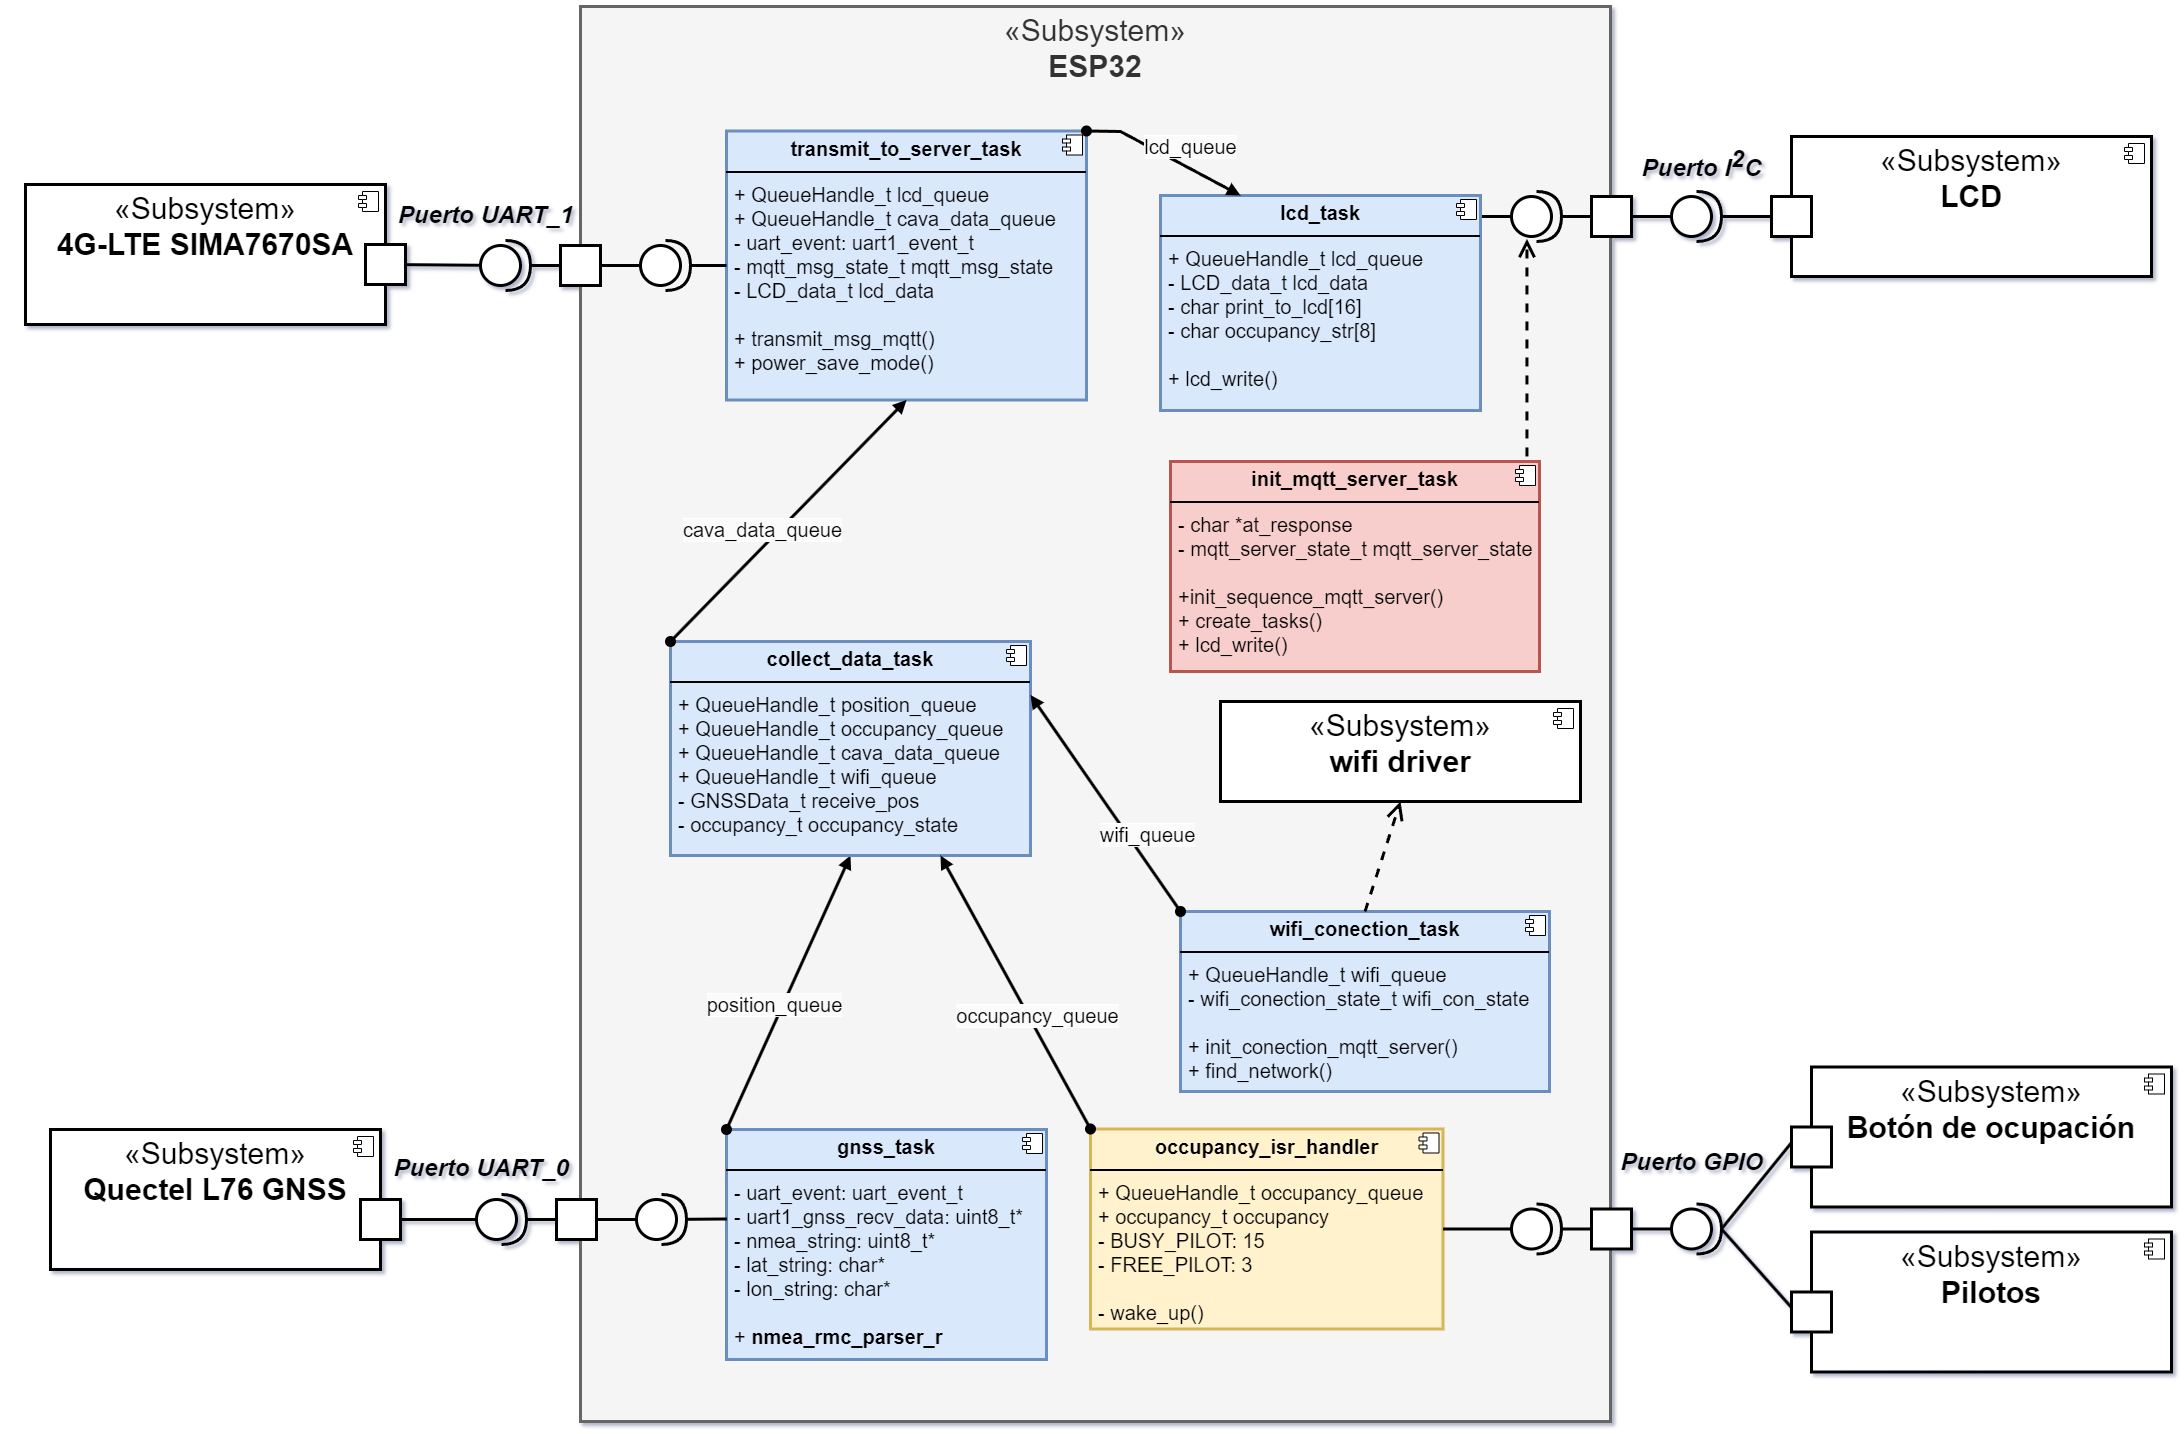
\includegraphics[width=1.1\textwidth]{./Figures/Arquitectura_firmware_TFE_GNSS.png}
	\caption{Arquitectura del firmware.}
	\label{fig:arq_firmware}
\end{figure}

En el diagrama de la figura~\ref{fig:arq_firmware} se presentan las los componentes de firmware más relevantes del sistema y la forma en que interactúan entre ellos. A continuación, se describe la funcionalidad d ecada componente del firmware:

\begin{enumerate}
	\item El firmware inicia con la tarea \textit{init\_mqtt\_server\_task()}, resaltada con color rojo, la cual se encarga de tres funciones primordiales: realizar la inicialización de los servicios MQTT que proporciona el módulo 4G (SIM A7670SA), realizar la conexión con el \textit{Broker} MQTT remoto y, si todo sale bien, desencadena la creación de las demás tareas del sistema. Esta tarea utiliza líneas de comandos AT para comunicarse con el módulo 4G.
	
	\item Tarea \textit{collect\_data\_task()}, se encarga de recibir a través de colas, la información relacionada con la ocupación y la posición de la cava, dicha información proveniente de la tarea \textit{gnss\_task()} y del manejador de interrupciones \textit{occupancy\_isr\_handler()}, respectivamente. Cuando esta tarea obtiene la información mencionada, las transmite a la tarea \textit{transmit\_to\_server\_task()}, a través de la cola \textit{cava\_data\_queue}.
	
	\item Manejador de interrupción \textit{occupancy\_isr\_handler()}, resaltada con color amarillo, es la función que se ejecuta siempre que ocurra una interrupción debida a los botones de ocupación de la cava, a saber, ocupado-desocupado. Este manejador de interrupción detecta qué botón se presionó y comunica a la tarea \textit{collect\_data\_task()} el estado de ocupación, a través de la cola \textit{occupancy\_queue}. Además, esta tarea genera una acción de \textit{wakeup} del sistema cuando se encuentra en modo ahorro de energía. 	
	
	\item Tarea \textit{gnss\_task()}, se encarga primordialmente de detectar la recepción de una trama NMEA del tipo GNRMC, lo que asegura que la posición ha sido calculada con señales de dos o más constelaciones satelitales; en este caso, GPS y BeiDou. La detección de tramas se realiza a través de interrupciones del módulo UART de la ESP32. Esta tarea descarta todas las tramas que no sean compatibles con el estándar NMEA y todas las que no sean del tipo GNRMC. Además, se encarga de la extracción de la información de las tramas RMC a través de la función \textit{nmea\_rmc\_parser\_r()}. Esta última es una implementación de tipo \textit{thread-safe} para asegurar la compatibilidad con FreeRTOS, ya que permite la multitarea. Además, comunica la posición actual a la tarea \textit{collect\_data\_task()}, a través de la cola \textit{position\_queue}. Por último, esta tarea verifica si la posición no ha cambiado en los últimos 5 minutos, en caso de no cambiar, colocará al sistema completo en modo ahorro de energía. 
		
	\item Tarea \textit{transmit\_to\_server\_task()}, se encarga de ejecutar la secuencia de transmisión de datos a través del protocolo MQTT, con el módulo 4G. La comunicación entre microcontrolador y el módulo se realiza a través de comandos AT. Esta tarea recibe los datos provenientes de la tarea \textit{collect\_data\_task()}, los transmite con la función \textit{transmit\_msg\_mqtt()}. Al finalizar, construye un paquete de información con los datos de ocupación, posición y resultado de la transmisión MQTT, para ser transferido a través de la cola \textit{lcd\_queue} hacia la tarea \textit{lcd\_task()}. 
		
	\item Tarea \textit{lcd\_task()} se encarga de administrar adecuadamente el acceso a los recursos de la pantalla LCD, para evitar sobrescritura o pérdida de información relevante que deba ser mostrada a través de la pantalla LCD. 
\end{enumerate}



\subsection{Implementación del firmware}
\label{sec:implementacion_firmware}

El firmware se implementó en el \textit{framework} ESP-IDF desarrollado por la empresa ESPRESSIF, para las series de SoCs ESP32, ESP32-S y ESP32-C. Este \textit{framework} proporciona un SDK apto para el desarrollo de cualquier aplicación genérica en estas plataformas, a partir de lenguajes de programación C y C++. Además, está optimizado para para aplicaciones de Internet de las Cosas (IoT, del inglés \textit{Internet of Things}). 

También se utilizó el entorno de desarrollo (IDE) \textit{PlatformIO}, que se ejecuta como una extensión nativa en el IDE de \textit{Visual Studio Code}. \textit{PlatformIO} permite usar todas las funcionalidades de ESP-IDF de una manera fiable y ágil, sin enmascarar funcionalidades o configuraciones avanzadas del \textit{framework}. Además, permite ejecutar las versiones mas estables de ESP-IDF, proporciona soporte por la comunidad de desarrolladores, es multiplataforma y de software libre. 

Para la implementación del firmware se utilizó el lenguaje de programación C y se implementó el sistema operativo en tiempo real FreeRTOS. Una ventaja importante que ofrece ESP-IDF es que está desarrollado sobre FreeRTOS, por tanto, el firmware se ejecuta nativamente en este.

Por petición del cliente, la codificación correspondiente al firmware no podrá ser mostrada, sin embargo, se empleará pseudocódigo para sustentarla y no comprometer la calidad del trabajo desarrollado. 

\subsubsection{Flujo general del firmware}

Gracias a la implementación en FreeRTOS, el firmware tiene la capacidad de ejecutar multitarea. El flujo general del programa se muestra en las figuras \ref{fig:flujo_firmware_1}, \ref{fig:flujo_firmware_2} y \ref{fig:flujo_firmware_3}. Como se puede ver en dicho diagrama y en el diagrama de la arquitectura (ver figura \ref{fig:arq_firmware}), las diferentes tareas se ejecutan una independiente de la otra. Sin embargo, existe un flujo de información que se sucede de una tarea a otra. Como mecanismo de comunicación entre tareas, se utilizan las colas. Este comportamiento del firmware es relevante desde el punto de vista en que el sistema puede estar recibiendo, procesando y transmitiendo datos de posicionamiento de manera casi concurrente. 

\begin{figure}
	\centering
	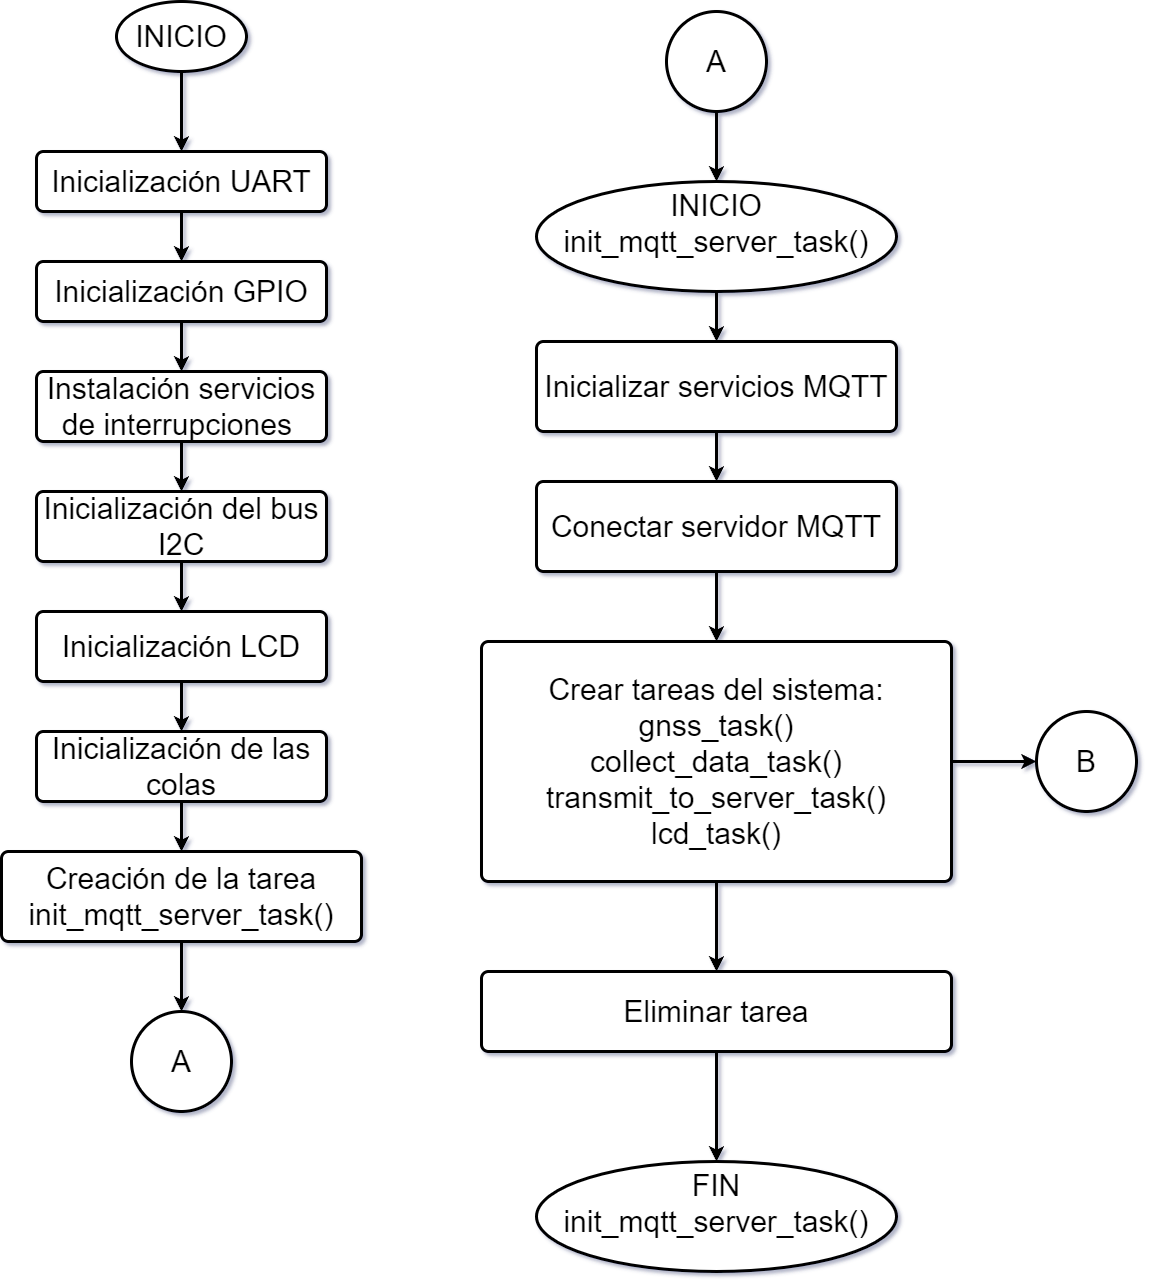
\includegraphics[width=.8\textwidth]{./Figures/Diagrama_flujo_firmware_TFE_CESE_Part_1.png}
	\caption{Diagrama de flujo del firmware (parte 1).}
	\label{fig:flujo_firmware_1}
\end{figure}

\begin{figure}
	\centering
	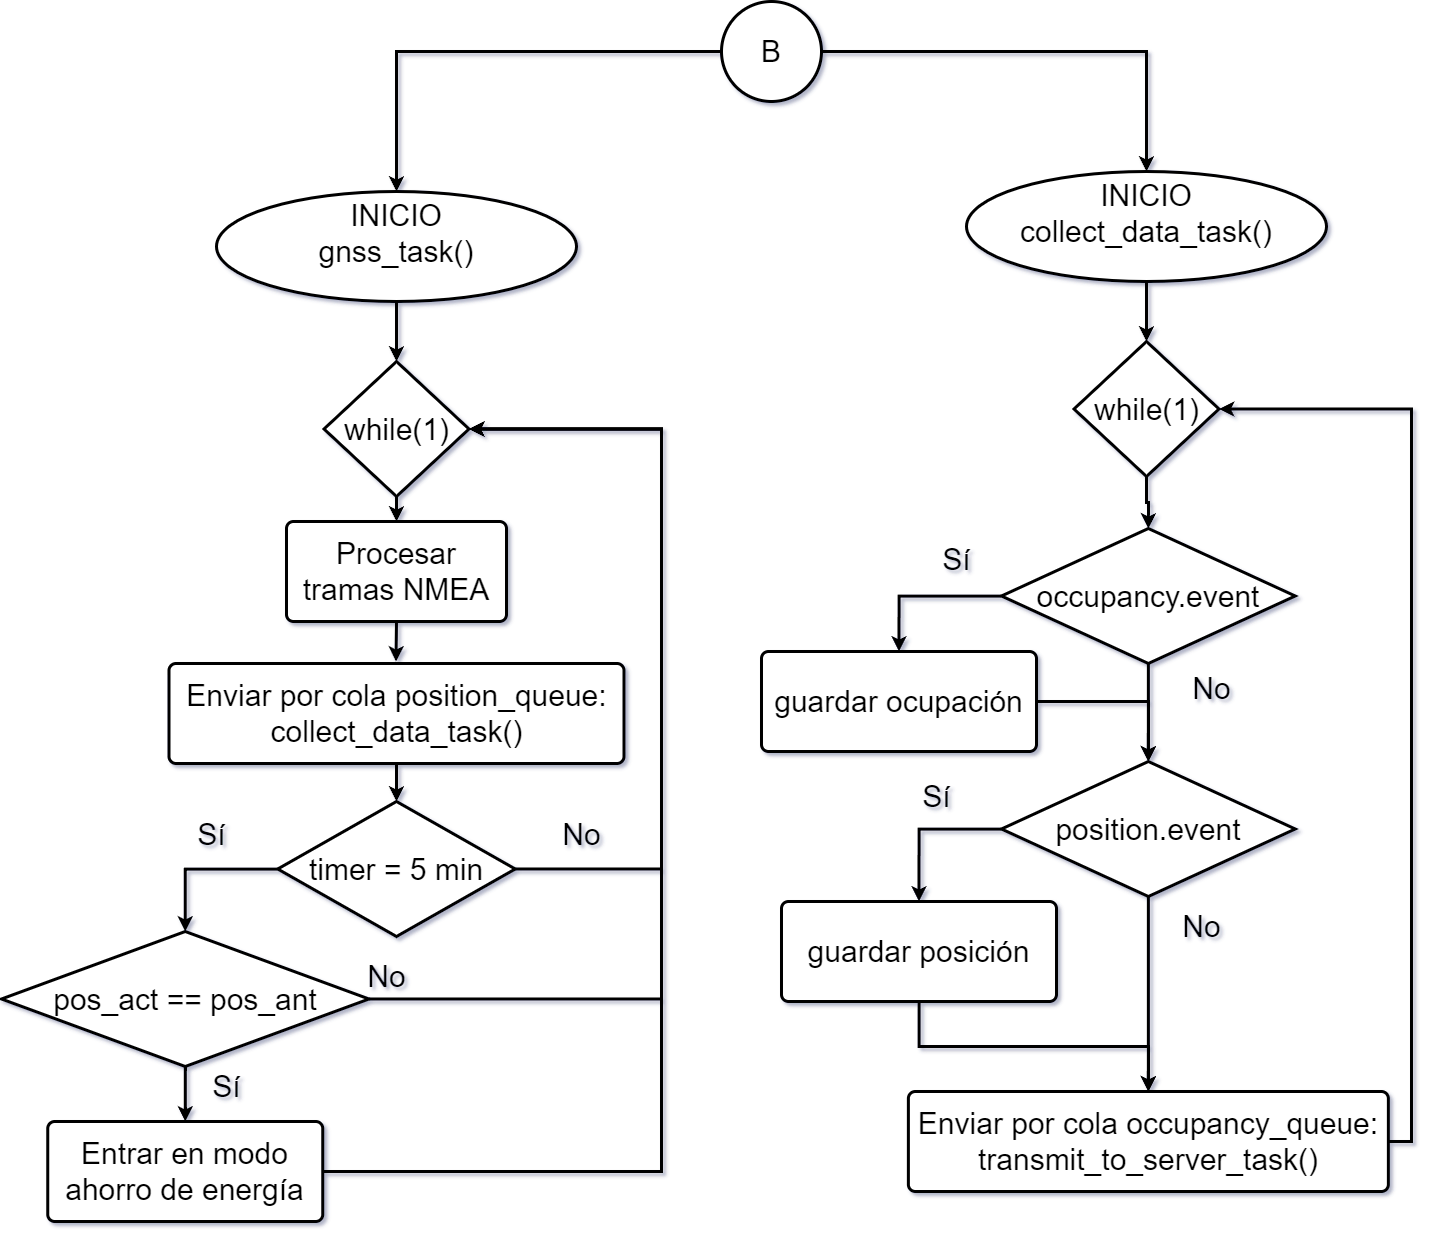
\includegraphics[width=.8\textwidth]{./Figures/Diagrama_flujo_firmware_TFE_CESE_Part_2.png}
	\caption{Diagrama de flujo del firmware (parte 2).}
	\label{fig:flujo_firmware_2}
\end{figure}

\begin{figure}
	\centering
	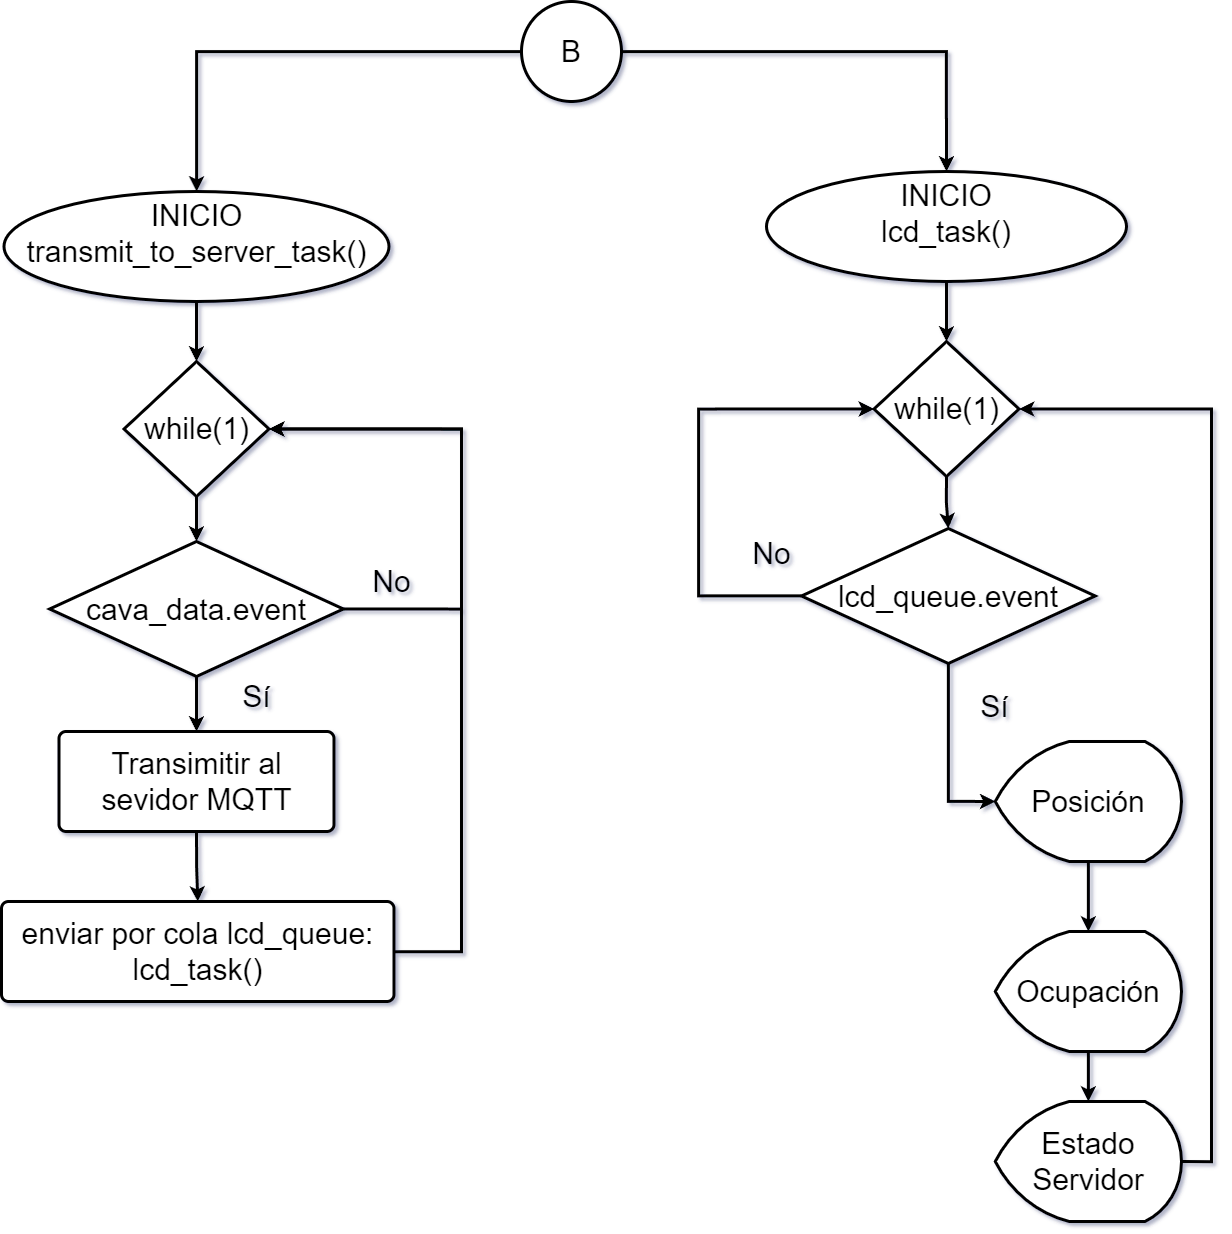
\includegraphics[width=.8\textwidth]{./Figures/Diagrama_flujo_firmware_TFE_CESE_Part_3.png}
	\caption{Diagrama de flujo del firmware (parte 3).}
	\label{fig:flujo_firmware_3}
\end{figure}


\subsubsection{Implementación de las tareas del sistema}

En los códigos, \ref{cod:init_mqtt_server_task}, \ref{cod:gnss_task}, \ref{cod:occupancy_isr_handler}, \ref{cod:collect_data_task}, \ref{cod:transmit_to_server_task} y \ref{cod:lcd_task} se presenta la implementación en pseudocódigo de cada una de las tareas principales del firmware. 


\begin{lstlisting}[label=cod:init_mqtt_server_task, caption=Pseudocódigo de la función init\_mqtt\_server\_task().] 

init_mqtt_server_task()
{
	while ("READY" == SIM_A7670SA)
		Esperar
	Inicalizar servicios MQTT en SIM_A7670SA
	while (4 == intentos)
		Conectar con Broker MQTT en la nube
		if ("OK" == Conexion_Servidor)
			Crear tareas: 
				gnss_task()
				collect_data_task()
				transmit_to_server_task()
				lcd_task()
			Eliminar: init_mqtt_server_task
			break
		else
			Reportar por LCD: Falla conexion Broker
			Eliminar: init_mqtt_server_task
}

\end{lstlisting}

 


\begin{lstlisting}[label=cod:gnss_task, caption=Pseudocódigo de la función gnss\_task().] 

gnss_task()
{
	while (1)
		if (DATA == envento_UART_0)
			Procesar trama: 
				posicion_actual = nmea_rmc_parser_r()
			Enviar por cola position_queue: posicion_actual
			if (Temporizar 5)
				if (posicion_anterior == posicion_actual)
					sleep_mode: Modulo_celular
					sleep_mode: Modulo_GNSS
					sleep_mode: ESP32
					
		posicion_anterior = posicion_actual
}

\end{lstlisting}

 


\begin{lstlisting}[label=cod:occupancy_isr_handler, caption=Pseudocódigo de la función occupancy\_isr\_handler().] 

occupancy_isr_handler()
{
	Capturar boton presionado
	switch (bonton)
		case boton_libre: 
			Setear los pilotos como libre
			Enviar por cola occupancy_queue: "Libre"
		
		case boton_ocupado:
			Setear los pilotos como ocupado
			Enviar por cola occupancy_queue: "Ocupado"	
}

\end{lstlisting}

 

\begin{lstlisting}[label=cod:collect_data_task, caption=Pseudocódigo de la función collect\_data\_task().] 

collect_data_task()
{
	while (1)
		if (DATA == occupancy_queue.event)
			datos_cava.occupancy = occupancy
			
		if (DATA == position_queue.event)
			datos_cava.position = position
		
		Enviar por cola cava_data_queue: datos_cava		
}

\end{lstlisting}

 

\begin{lstlisting}[label=cod:transmit_to_server_task, caption=Pseudocódigo de la función transmit\_to\_server\_task().] 

transmit_to_server_task()
{
	posicion_anterior
	while (1)
		if (DATA == cava_data_queue.event)
			Transmitir al Broker MQTT: 
				transmision_state = transmit_msg_mqtt()
			Enviar por cola lcd_queue: cava_data+transmision_state
}

\end{lstlisting}

 

\begin{lstlisting}[label=cod:lcd_task, caption=Pseudocódigo de la función lcd\_task().] 

lcd_task()
{
	while (1)
		if (DATA == lcd_queue.event)
			Escribir_LCD: position.lat
			Escribir_LCD: position.long
			Escribir_LCD: position.time
			Escribir_LCD: position.val // Validez de la posicion
			Escribir_LCD: occupancy
			Escribir_LCD: server_state
}

\end{lstlisting}



\subsubsection{Otros componentes del firmware}

Además de las tareas y funciones descritas en la sección \ref{fig:arq_firmware}, fue necesario implementar varios componentes de firmware. Sin embargo, por ser los más relevantes, se mencionan los siguientes:

\begin{enumerate}
	\item Un driver para el manejo de la pantalla \textit{LCD RGB Backlight} de 16x2 que se llamó \textit{lcd\_i2c\_grove.h}. Esta pantalla presenta interfaz de comunicación I2C, para reducir la cantidad de pines utilizados por el microcontrolador. Este driver presenta las funciones descritas en el código \ref{lst:driver_lcd}.
	
	\item Una función para inicializar los servicios MQTT en el módulo SIM A7670SA y conectarse al \textit{Broker} MQTT, que se llamó \textit{init\_sequence\_mqtt\_server()}. Esta función implementa comandos AT específicos para el módulo en mención. Retorna el estado de conexión con el \textit{Broker} MQTT o en su defecto los errores encontrados en el proceso. En el código \ref{cod:init_sequence_mqtt_server} se muestra el pseudocódigo que describe su funcionamiento.
	
	\item Una función para encapsular la funcionalidad de transmitir al \textit{Broker} MQTT una vez se ha establecido la conexión. Esta es \textit{transmit\_msg\_mqtt()}. Esta función implementa comandos AT específicos del módulo SIM A7670SA y retorna el estado de transmisión del mensaje. En el código \ref{cod:transmit_msg_mqtt} se muestra el pseudocódigo que describe su funcionamiento.
	
	\item Una función que permite extraer la información de las cadenas tipo GNRMC recibidas por el módulo Quectel L76. Esta es una función de tipo \textit{thread-safe} para facilitar la multitarea, que se nombró como \textit{nmea\_rmc\_parser\_r()}. En el código \ref{cod:nmea_rmc_parser_r} se muestra el pseudocódigo que describe su funcionamiento.
\end{enumerate}


\begin{lstlisting}[label={lst:driver_lcd}, caption={Funciones principales del driver LCD.}] 

/**
 * @brief Esta funcion incializa las funcionalidades I2C y la configuracion de escritura de la pantalla
 */
void lcd_init();

/**
 * @brief Esta funcion escribe en la pantalla LCD el texto deseado.
 * 
 * @param row: Columna desde la cual se inica la escritura
 * @param column: Fila sobre la cual se desea escribir
 * @param str: Texto que se desea escribir
 */
void lcd_write(uint8_t row, uint8_t column, char *str);

/**
 * @brief Esta funcion limpia o borra todos los caracteres de la pantalla LCD.
 */
void lcd_clear();

/**
 * @brief Esta funcion cambia el color de fondo de la pantalla LCD segun el modelo de color RGB.
 * 
 * @param r: valor para cantidad de color rojo.
 * @param g: valor para cantidad de color verde.
 * @param b: valor para cantidad de color azul.
 */
void lcd_set_RGB(unsigned char r, unsigned char g, unsigned char b);

\end{lstlisting}

 


\begin{lstlisting}[label=cod:init_sequence_mqtt_server, caption=Pseudocódigo de la función init\_sequence\_mqtt\_server().] 

init_sequence_mqtt_server(uart_event_t uart1_event, char * at_response)
{
  Enviar AT: iniciar el servicio MQTT
  if ("OK" == respuesta)
      Enviar AT: adquirir cliente MQTT
      if ("OK" == respuesta)
          Enviar AT: conectar con Broker MQTT
	      if ("OK" == respuesta)
	          return: MQTT_SERVER_OK
	      else 
	          return: MQTT_FAIL_INIT_SERVER
      else
          return: MQTT_FAIL_ADQ_CLIENT
  else
      return: MQTT_FAIL_INIT_SERVICE	
}

\end{lstlisting}
 




\begin{lstlisting}[label=cod:transmit_msg_mqtt, caption=Pseudocódigo de la función init\_sequence\_mqtt\_server().] 

transmit_msg_mqtt(char * mqtt_payload, char * topic, uart_event_t uart1_event, char * at_response)
{
	Enviar AT: configurar topic
	if ("OK" == respuesta)
		Enviar AT: cargar payload
		if ("OK" == respuesta)
			Enviar AT: publicar
			if ("OK" == respuesta)
				return: MQTT_MSG_OK
			else
				return: MQTT_MSG_FAIL
		else
			return: MQTT_MSG_FAIL
	else
		return: MQTT_TOPIC_FAIL
}

\end{lstlisting}

 


\begin{lstlisting}[label=cod:nmea_rmc_parser_r, caption=Pseudocódigo de la función nmea\_rmc\_parser\_r().] 

nmea_rmc_parser_r(char *nmeaString, GNSSData_t *gnssData)
{
	Verificar trama inicia con "$"
	if ("$" == token_0)
		Dividir trama en tokens por ","
		Verificar que el primer token sea "GNRMC"
		if("GNRMC" == token_1)
			time = token_2 
			if("A" == token_3)
				latitud = convertir_DMS_to_DD(token_4, token_5)
				longitud = convertir_DMS_to_DD(token_6, token_7)
			else
				return: NMEA_NO_VALID			
			 
		else
			return: NMEA_NO_RMC
	else
		return: NMEA_NO_VALID
}

\end{lstlisting}




%----------------------------------------------------------------------------------------
%	SECTION 4
%----------------------------------------------------------------------------------------
\section{Diseño e implementación de la interfaz web}

En esta sección se presentan las consideraciones de diseño y la metodología de implementación de la interfaz web.

\subsection{Diseño de la interfaz web}

Para el diseño de la interfaz web, se tuvo en cuenta satisfacer la historia de usuario descrita en la planificación de este trabajo y que motiva al desarrollo de este componente: 

\textit{Como usuario final quiero ver una página web con un mapa que me muestre la posición en tiempo real de todas las cavas y su estado de ocupación para realizar un seguimiento de estas y organizar la logística del reparto de productos en la cadena de frío.}

De acuerdo con lo anterior y con el análisis de la sección \ref{sec:mapas_web}, se escogió la biblioteca \textit{leaflet.js}\footnote{Documentación en: \url{https://leafletjs.com/index.html}} para la creación de mapas en la web, debido a que la empresa Cloud Technologys SAS, integra sus desarrollos web con tecnologías web con JavaScript y a que en la etapa de desarrollo del producto no se requerirá incurrir en gastos para el despliegue en pruebas o en entornos relevantes. 

El desarrollo de la aplicación web se llevó a cabo siguiendo la arquitectura mostrada en la figura \ref{fig:arq_mqtt}. En ella se puede apreciar 

\begin{figure}[htbp]
	\centering
	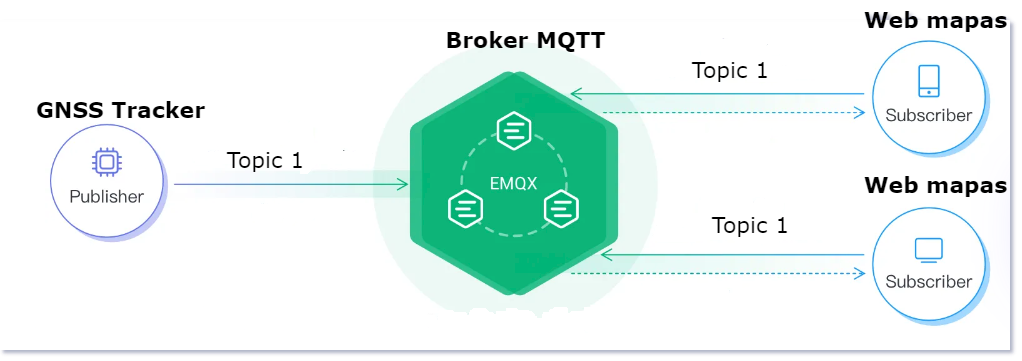
\includegraphics[width=.9\textwidth]{./Figures/arquitectura_MQTT.png}
	\caption{Arquitectura MQTT \protect\footnotemark.}
	\label{fig:arq_mqtt}
\end{figure}
\footnotetext{Imagen adaptada de: \url{https://www.emqx.com/en/blog/mqtt-5-introduction-to-publish-subscribe-model}}

En esta arquitectura, el centro de la comunicación es el \textit{Broker} MQTT, donde se centralizan los mensajes de los \textit{publishers} para ser transmitidos hacia los dispositivos \textit{subscribers}, a través de canales específicos, llamados tópicos. El \textit{Broker} MQTT es responsable de recibir conexiones iniciadas por el cliente y reenviar mensajes enviados por el cliente a otros clientes elegibles \citep{MasteringMQTT}. 

Para este trabajo, se utilizó el \textit{Broker} EMQX\footnote{Documentación en: \url{https://www.emqx.io/}}, que es utilizado para aplicaciones de IoT \citep{MasteringMQTT}.

La aplicación web al igual que el hardware desarrollado, son clientes del \textit{Broker} EMQX. El hardware es el encargado de publicar mensajes con los datos de posicionamiento, estado ocupación, validez de la posición, la hora y la referencia de la cava. Por otro lado, la aplicación web recibe dichos datos y los hace visibles al usuario a través un mapa y otros elementos de visualización web. El usuario final puede visualizar   

\subsection{Implementación de la interfaz web}

Para la implementación de la interfaz web, se utilizaron las siguientes tecnologías: 

\begin{itemize}
	\item HTML: Se utiliza para estructurar la página web.
	\item CSS (Bootstrap): Se usa para dar estilo a la página, para crear un diseño \textit{responsiv} y facilitar la implementación ya que cuenta con componentes predefinidos.
	\item lenguaje de programación JavaScript, características y bibliotecas de éste. A continuación, se detallan las más relevantes para este trabajo: 
		\begin{itemize}
			\item jQuery: Biblioteca de JavaScript utilizada para facilitar la manipulación del DOM, eventos y AJAX.
			\item Leaflet.js: Biblioteca de JavaScript para mapas interactivos.
			\item mqtt.js: Biblioteca de JavaScript para conectarse a un broker MQTT, permitiendo la comunicación en tiempo real entre el navegador y el broker.
		\end{itemize}
	\item \textit{IDE Visual Studio Code} para realizar la codificación. 
	\item Docker como plataforma para la etapa de desarrollo, donde se ejecutó el EMQX.
	\item \textit{Broker} EMQX. 
\end{itemize}


\subsection{Metodología de la implementación}
\label{sec:met_web}

A continuación, se presenta el proceso llevado a cabo para la implementación de la interfaz web. 

\begin{enumerate}
	\item \textbf{Configuración Inicial:}
		\begin{itemize}
		\item Se diseñó la estructura de la página web usando HTML y Bootstrap. En este punto se utilizaron las bibliotecas necesarias para la funcionalidad del mapa y la conexión MQTT. En la figura \ref{} se observa la versión desarrollada por el autor. Además, en la figura \ref{} se muestra la versión implementada en el servidor de la empresa Cloud Technologys SAS, la cual fue migrada y ajustada por su equipo de desarrolladores web.
		\end{itemize}

	\item \textbf{Configuración del Mapa:}
		\begin{itemize}
		\item Con Leaflet.js se inicializa un mapa centrado en una posición predeterminada y se añade una capa de OpenStreetMap para mostrar el mapa base.
		\end{itemize}
		
	\item \textbf{Configuración de la Conexión MQTT:}
		\begin{itemize}
		\item Se configuran las opciones de conexión al broker MQTT, a saber URL del broker, credenciales de usuario, parámetro \textit{keepalive} y el parámetro \textit{connectTimeout}. Se establece la conexión con el \textit{Broker} utilizando mqtt.js. Por último, se realiza la suscripción  al tópico que recibe los datos de ubicación del dispositivo GNSS.
		\end{itemize}
	
	\item \textbf{Gestión de Mensajes:}
		\begin{itemize}
		\item Se define la función \textit{get\_cava\_data()} para procesar los mensajes recibidos del broker. Se convierten los mensajes a formato JSON y se extraen los datos de la cava. Se actualiza el mapa con la nueva posición de la cava, los demás datos actualizados y se muestra la ruta seguida.
		\end{itemize}
		
	\item \textbf{Actualización del Mapa:}
		\begin{itemize}
		\item Se elimina el marcador anterior y se añade un nuevo marcador en la nueva posición. Se actualiza la vista del mapa para centrarse en la nueva posición y se muestra la ruta recorrida por la cava utilizando una polilínea.
		\end{itemize}

\end{enumerate}


En el código \ref{cod:aplicacion_web} se muestra la implementación HTML de la interfaz web desarrollada por el autor, la cual sirvió de maqueta para que el equipo de desarrollo web de la empresa Cloud Technologys SAS lo implementara en sus servidores. Sin embargo, por petición del cliente, no es posible compartir el código implementado en sus servidores. 

Además, en el código \ref{cod:aplicacion_web_js}, se presenta la implementación de la dinámica de conexión del dispositivo y las funcionalidades necesarias para la inicialización del mapa y las conexiones 

\begin{lstlisting}[label=cod:aplicacion_web, caption=Pseudocódigo para la implementación HTML de la página web.] 

<!DOCTYPE html>
<html>
  <head>
    <title>Cava mapa</title>

    <link rel="stylesheet" href="https://stackpath.bootstrapcdn.com/bootstrap/4.5.2/css/bootstrap.min.css" crossorigin="anonymous">
    <script src="https://code.jquery.com/jquery-3.5.1.slim.min.js" crossorigin="anonymous"></script>
    <script src="https://cdn.jsdelivr.net/npm/@popperjs/core@2.5.3/dist/umd/popper.min.js" crossorigin="anonymous"></script>
    <script src="https://stackpath.bootstrapcdn.com/bootstrap/4.5.2/js/bootstrap.min.js" crossorigin="anonymous"></script>

    <link rel="stylesheet" type="text/css" href="leaflet.css" />
    
  </head>
  <body>

    <h1> GNSS Cava: </h1> <h2> Cava001 </h2> 

    <div class="container mt-4">
        <div class="row">
            <div class="col-md-4">
                <div class="card mb-3">
                    <div class="card-body">
                        <h5 class="card-title">Dispositivo: </h5>
                        <p class="card-text" id="cava_name">h</p>
                    </div>
                </div>
                <div class="card mb-3">
                    <div class="card-body">
                        <h5 class="card-title">Posicion: </h5>
                        <p class="card-text" id="lat"></p>
                        <p class="card-text" id="lng"></p>
                    </div>
                </div>
                <div class="card mb-3">
                    <div class="card-body">
                        <h5 class="card-title">Estado: </h5>
                        <p class="card-text" id="estado"></p>
                    </div>
                </div>
                <div class="form-group">
                    <label for="exampleSelect">Seleccionar cava</label>
                    <select class="form-control" id="cava_select">
                        <option>Cava_001</option>
                        <option>Cava_002</option>
                        <option>Cava_003</option>
                    </select>
                </div>
            </div>

            <div class="col-md-8">
                <div id="map"></div>
            </div>

        </div>
    </div>

    <script src="leaflet.js"></script>
    <script src="mqtt.min.js"></script>
    <script type="module" src="mapa.js"></script>
  </body>

</html>



\end{lstlisting}


\begin{lstlisting}[label=cod:aplicacion_web_js, caption=Implementación en javascript de la parte dinámica de la página web.] 

let map;
let marker;
let path = [];
let polyline
const home = { lat: 10.918982886682658, lng: -74.87194240611939 };
let current_cava_position;

const options = {
    clean: true, // retain session
    connectTimeout: 4000, // Timeout period
    clientId: 'web_app_cava_position',
    username: '*****',
    password: '****',
    Keepalive: 60,
};

const connectUrl = '*******';
const client = mqtt.connect(connectUrl, options);
const topic_cava = 'proyectoLuis/cava/datos';
let cava_data;

function init_map(){
    //map = L.map('cava_map').setView([home.lat, home.lng], 13);
    map = L.map('map').setView([home.lat, home.lng], 13);
    //OpenStreetMap 
    var tile_map = L.tileLayer('https://tile.openstreetmap.org/{z}/{x}/{y}.png', {
        maxZoom: 19,
        attribution: '&copy; <a href="http://www.openstreetmap.org/copyright">OpenStreetMap</a>'
    });

    tile_map.addTo(map)

    marker = L.marker([home.lat, home.lng]).addTo(map);
    marker.bindPopup("<b>Posicion</b>"+"<br>"+"lat: "+home.lat.toString()+
                     "<br>"+" lng: "+home.lng.toString()+
                     "<br> CD"
                    ).openPopup();
}

function get_cava_data(cava_data) {

    let latitude = parseFloat(cava_data.lat);
    let longitude = parseFloat(cava_data.long);

    return { lat: latitude, lng: longitude };
}

function set_cava_position_map(position){
    
    document.getElementById('lat').textContent = "Lat: "+position.lat.toString();
    document.getElementById('lng').textContent = "Lng: "+position.lng.toString();
    
    if (marker) {
        map.removeLayer(marker);
    }

    marker = L.marker([position.lat, position.lng]).addTo(map);
    var popup_info = "<b>Posicion</b>"+"<br>"+position.lat.toString()+", "+position.lng.toString();
    marker.bindPopup(popup_info).openPopup();

    path.push([position.lat, position.lng]);
/*
    if (path.length > 1) {
        map.removeLayer(rastro);
    }
        */

    var rastro = L.polyline(path, {color: 'blue'}).addTo(map);

    map.setView([position.lat, position.lng], 15);
}

init_map();

client.on('connect', function () {
    console.log('Conectado')
    // Subscribe to a topic
    client.subscribe(topic_cava, { qos: 0 }, function (err) {
        if (!err) {
            console.log('Suscrito')
        }
    })
});

client.on('reconnect', (error) => {
    console.log('reconectando:', error)
});

client.on('error', (error) => {
    console.log('Conexion fallida:', error)
});

client.on('message', (topic, message) => {

    //console.log('mensaje recibido', topic, current_cava_position)
    current_cava_position = get_cava_data(JSON.parse(message.toString()));
    set_cava_position_map(current_cava_position);
});

\end{lstlisting}


\begin{figure}[htbp]
	\centering
	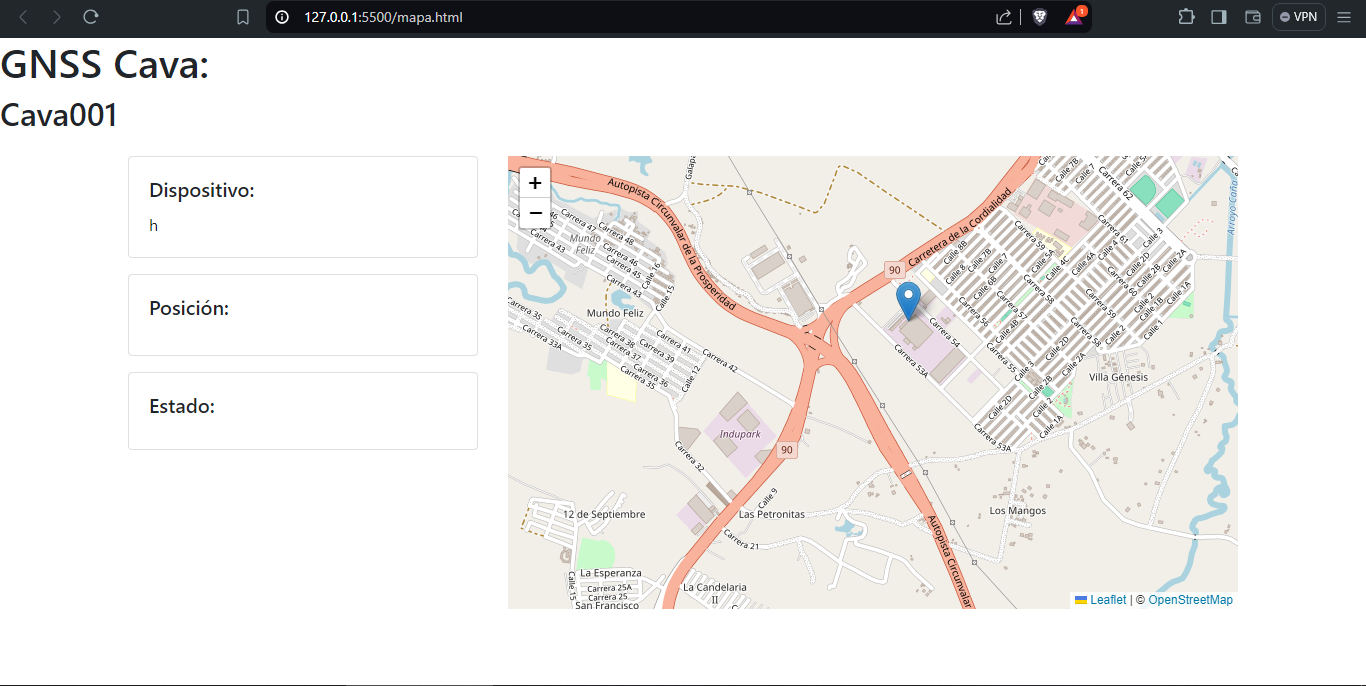
\includegraphics[width=1\textwidth]{./Figures/Mockup_web.png}
	\caption{Maqueta de la interfaz web.}
	\label{fig:mockup}
\end{figure}


\begin{figure}[htbp]
	\centering
	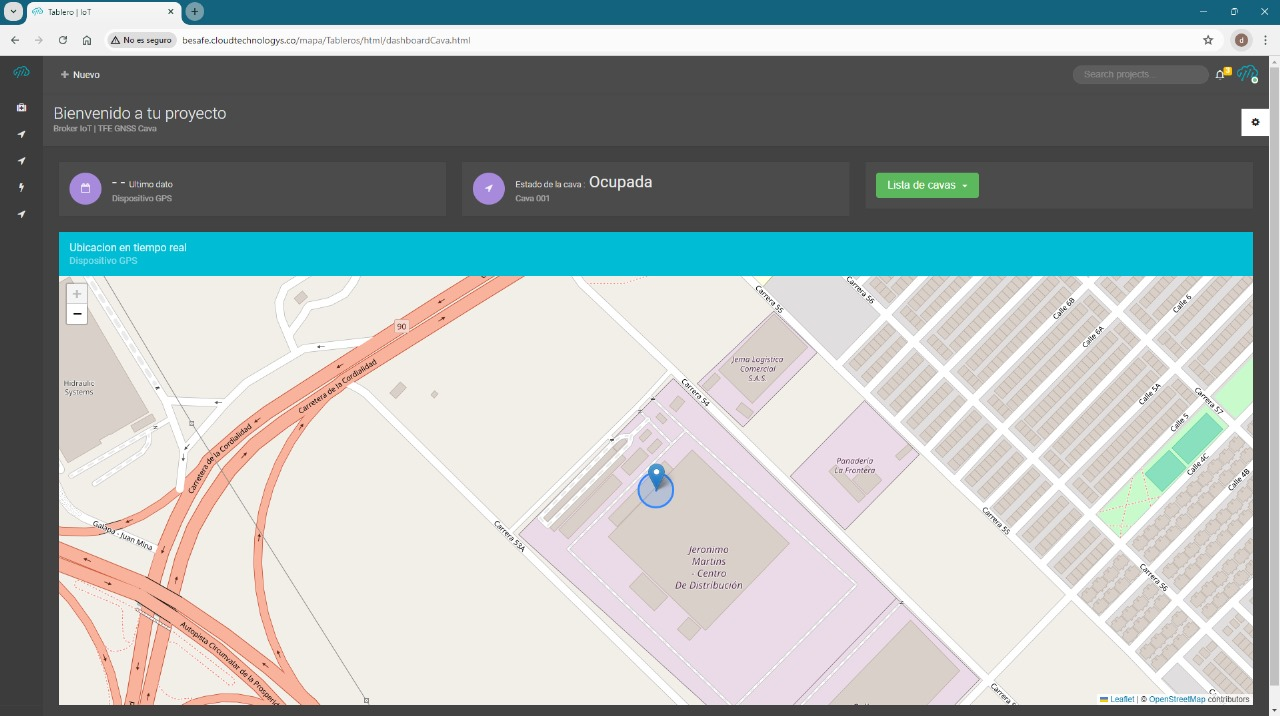
\includegraphics[width=1\textwidth]{./Figures/web_final.jpeg}
	\caption{Maqueta de la interfaz web.}
	\label{fig:web_final}
\end{figure}












\begin{comment}

\definecolor{mygreen}{rgb}{0,0.6,0}
\definecolor{mygray}{rgb}{0.5,0.5,0.5}
\definecolor{mymauve}{rgb}{0.58,0,0.82}

%%%%%%%%%%%%%%%%%%%%%%%%%%%%%%%%%%%%%%%%%%%%%%%%%%%%%%%%%%%%%%%%%%%%%%%%%%%%%
% parámetros para configurar el formato del código en los entornos lstlisting
%%%%%%%%%%%%%%%%%%%%%%%%%%%%%%%%%%%%%%%%%%%%%%%%%%%%%%%%%%%%%%%%%%%%%%%%%%%%%
\lstset{ %
  backgroundcolor=\color{white},   % choose the background color; you must add \usepackage{color} or \usepackage{xcolor}
  basicstyle=\footnotesize,        % the size of the fonts that are used for the code
  breakatwhitespace=false,         % sets if automatic breaks should only happen at whitespace
  breaklines=true,                 % sets automatic line breaking
  captionpos=b,                    % sets the caption-position to bottom
  commentstyle=\color{mygreen},    % comment style
  deletekeywords={...},            % if you want to delete keywords from the given language
  %escapeinside={\%*}{*)},          % if you want to add LaTeX within your code
  %extendedchars=true,              % lets you use non-ASCII characters; for 8-bits encodings only, does not work with UTF-8
  %frame=single,	                % adds a frame around the code
  keepspaces=true,                 % keeps spaces in text, useful for keeping indentation of code (possibly needs columns=flexible)
  keywordstyle=\color{blue},       % keyword style
  language=[ANSI]C,                % the language of the code
  %otherkeywords={*,...},           % if you want to add more keywords to the set
  numbers=left,                    % where to put the line-numbers; possible values are (none, left, right)
  numbersep=5pt,                   % how far the line-numbers are from the code
  numberstyle=\tiny\color{mygray}, % the style that is used for the line-numbers
  rulecolor=\color{black},         % if not set, the frame-color may be changed on line-breaks within not-black text (e.g. comments (green here))
  showspaces=false,                % show spaces everywhere adding particular underscores; it overrides 'showstringspaces'
  showstringspaces=false,          % underline spaces within strings only
  showtabs=false,                  % show tabs within strings adding particular underscores
  stepnumber=1,                    % the step between two line-numbers. If it's 1, each line will be numbered
  stringstyle=\color{mymauve},     % string literal style
  tabsize=2,	                   % sets default tabsize to 2 spaces
  title=\lstname,                  % show the filename of files included with \lstinputlisting; also try caption instead of title
  morecomment=[s]{/*}{*/}
}

Se puede agregar código o pseudocódigo dentro de un entorno lstlisting con el siguiente código:

\begin{verbatim}
\begin{lstlisting}[caption= "un epígrafe descriptivo"]
	las líneas de código irían aquí...
\end{lstlisting}
\end{verbatim}

A modo de ejemplo:

\begin{lstlisting}[label=cod:vControl,caption=Pseudocódigo del lazo principal de control.]  % Start your code-block

#define MAX_SENSOR_NUMBER 3
#define MAX_ALARM_NUMBER  6
#define MAX_ACTUATOR_NUMBER 6

uint32_t sensorValue[MAX_SENSOR_NUMBER];		
FunctionalState alarmControl[MAX_ALARM_NUMBER];	//ENABLE or DISABLE
state_t alarmState[MAX_ALARM_NUMBER];						//ON or OFF
state_t actuatorState[MAX_ACTUATOR_NUMBER];			//ON or OFF

void vControl() {

	initGlobalVariables();
	
	period = 500 ms;
		
	while(1) {

		ticks = xTaskGetTickCount();
		
		updateSensors();
		
		updateAlarms();
		
		controlActuators();
		
		vTaskDelayUntil(&ticks, period);
	}
}
\end{lstlisting}

\end{comment}

